\chapter{Store Sales Prediction: Forecasting}
\label{cap:forecasting}

% =============================================================================
\section{Introduzione e Obiettivo del Forecasting}
\label{sec:intro_forecasting}
% =============================================================================

Nel presente capitolo viene sviluppata un'analisi avanzata di \textbf{Analisi delle Serie Temporali e Previsione (\emph{Forecasting})} applicata al dataset \textit{Store Sales - Time Series Forecasting}, reso disponibile sulla piattaforma Kaggle. L'obiettivo primario di questo studio è analizzare l'andamento storico dei volumi di vendita al dettaglio (\texttt{sales}) per costruire modelli statistici e econometrici in grado di anticipare con elevata accuratezza i trend commerciali futuri.

Seguendo rigorosamente le indicazioni metodologiche e le linee guida dei docenti (in analogia con i progetti di predizione finanziaria e di analisi dei trend storici presenti in letteratura), anziché utilizzare il file di test originale della competizione — il quale risulta sprovvisto dei valori di \textit{ground truth} essendo una sfida aperta — il dataset di training originario è stato sottoposto a una suddivisione sequenziale temporale:
\begin{enumerate}
    \item \textbf{Set di Addestramento (\emph{Training Set}):} corrispondente all'80% iniziale delle osservazioni temporali (dal 2013 fino alle soglie del 2016), utilizzato per l'identificazione dei pattern, l'istimazione dei parametri autoregressivi e l'ottimizzazione dei modelli.
    \item \textbf{Set di Valutazione (\textit{Test Set}):} corrispondente al restante 20% finale delle osservazioni (periodo recente), impiegato per testare rigorosamente la capacità di generalizzazione fuori campione dei modelli stimati e calcolare le metriche d'errore finali.
\end{enumerate}

% =============================================================================
\section{Fase di ETL e Preparazione dei Dati}
\label{sec:etl_forecasting}
% =============================================================================

Il dataset originario si presenta con una granularità estremamente fine (oltre 3 milioni di record), in quanto registra le vendite giornaliere disaggregate per i $54$ punti vendita (\texttt{store\_nbr}) e le $33$ famiglie di prodotti (\texttt{family}). Per ricondurre il problema a una serie temporale univariata solida e coerente con l'architettura dei modelli previsionali classici, è stata eseguita una rigorosa fase di pre-elaborazione (\textit{Extract, Transform, Load}):

\begin{enumerate}
    \item \textbf{Conversione e Indicizzazione Temporale:} La colonna \texttt{date} è stata convertita nel formato standard \texttt{datetime} di Pandas ed impostata come indice temporale del DataFrame.
    \item \textbf{Aggregazione Globale delle Vendite:} I dati giornalieri sono stati raggruppati mediante operatore di somma (\texttt{groupby('date')['sales'].sum()}), ottenendo il volume complessivo delle vendite giornaliere dell'intera catena di negozi nel periodo 2013--2017.
    \item \textbf{Controllo della Continuità del Calendario:} L'intera serie è stata risampionata a frequenza giornaliera continua (\texttt{asfreq('D')}) per identificare e trattare correttamente eventuali giorni mancanti o festività, imputando i valori nulli residui o azzerando i volumi nei giorni di chiusura totale dei punti vendita.
\end{enumerate}

\begin{figure}[H]
    \centering
    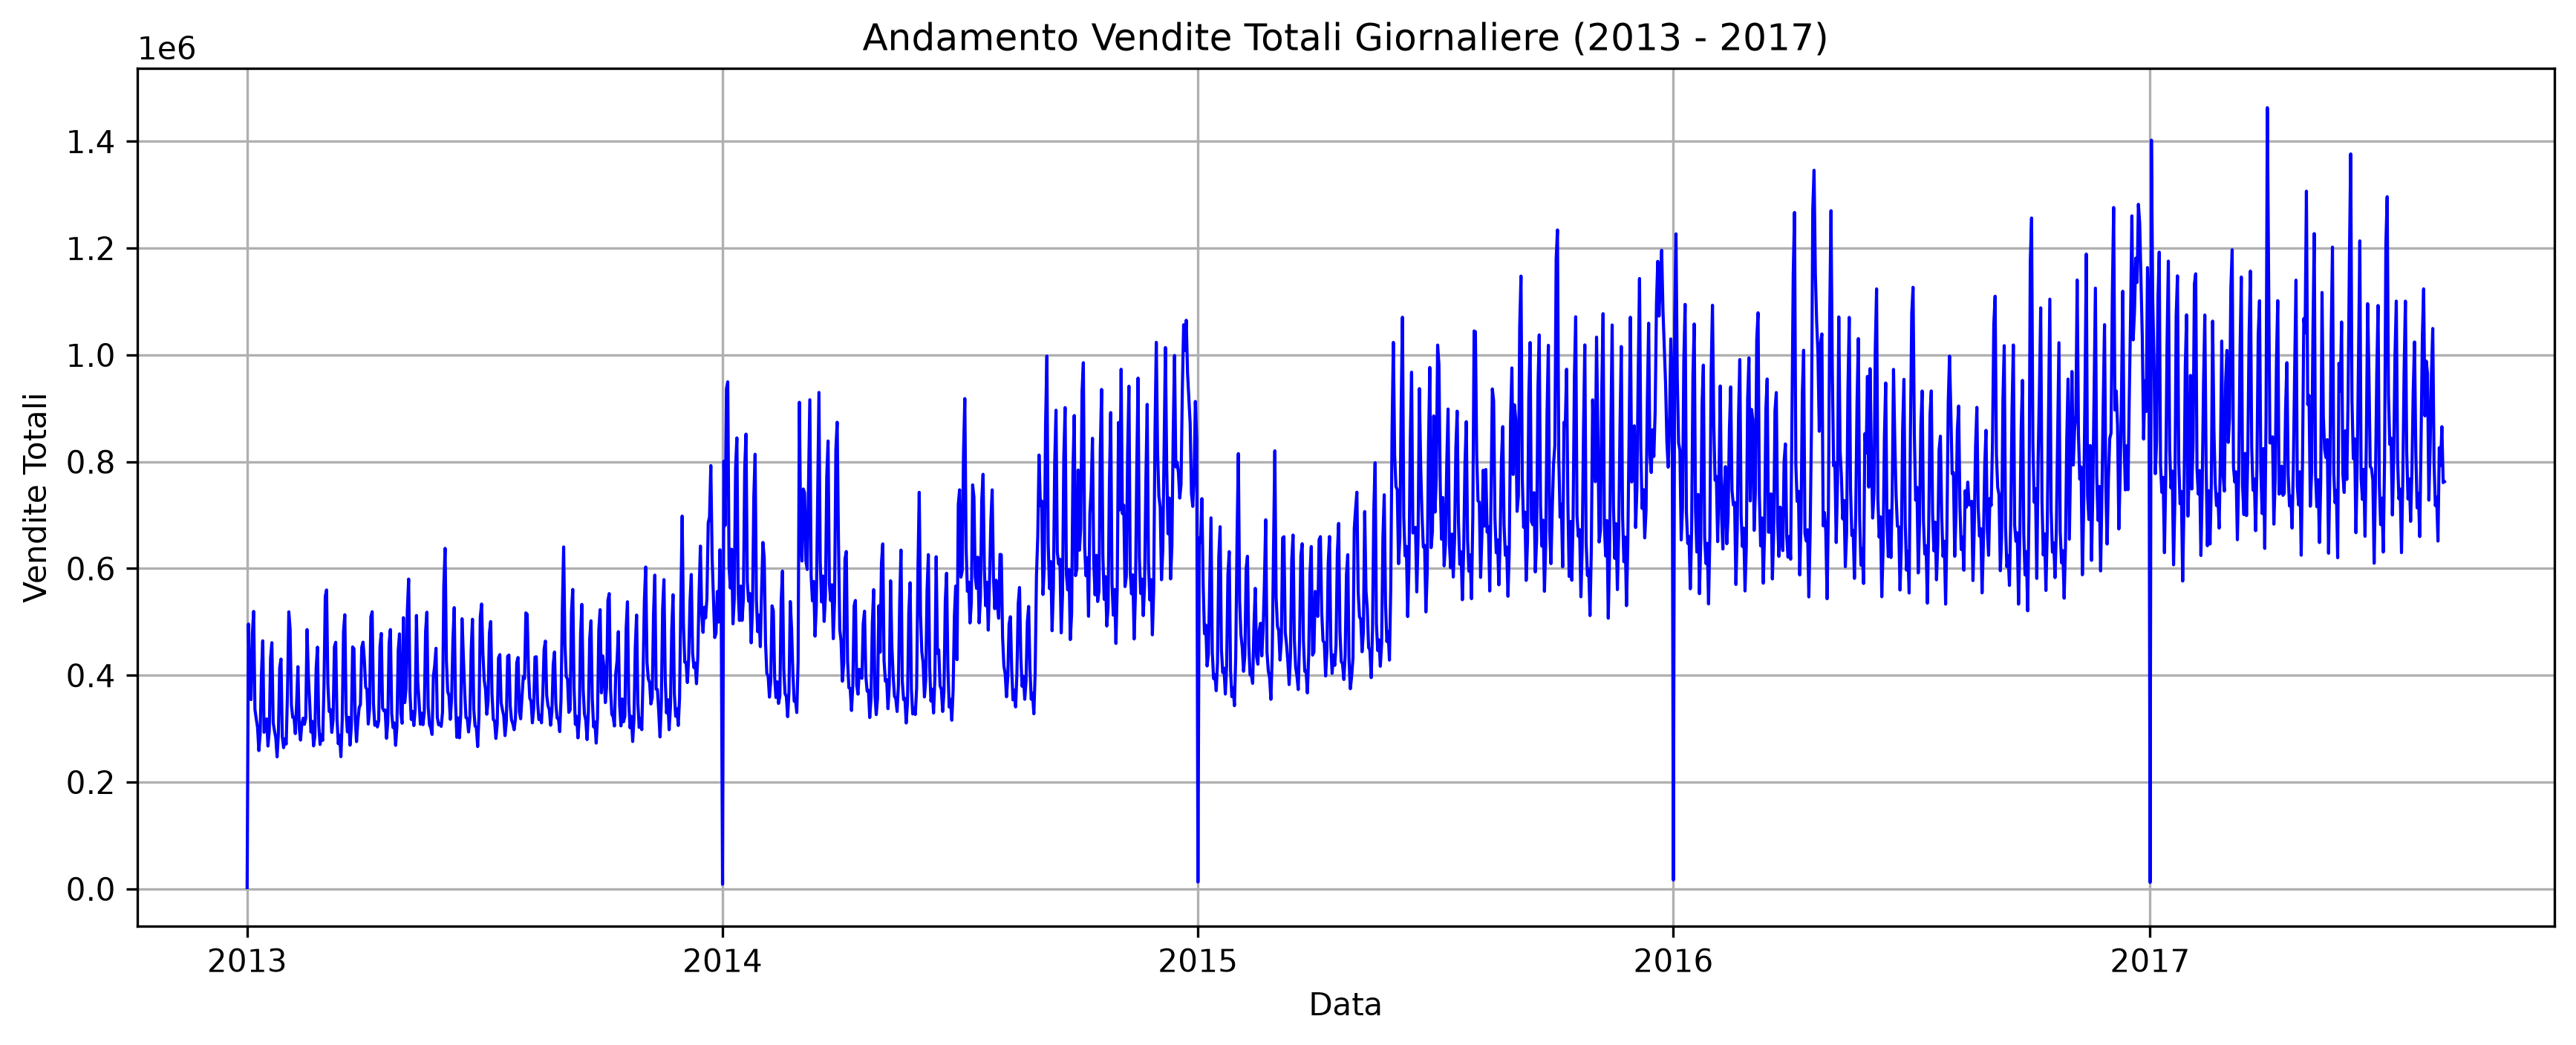
\includegraphics[width=\textwidth]{forecasting/images/fig01_andamento_vendite.png}
    \caption{Andamento temporale delle vendite totali giornaliere aggregate ($N = 1.684$ giorni, 2013--2017).}
    \label{fig:vendite_totali_forecasting}
\end{figure}

L'analisi esplorativa visiva della serie temporale (Figura~\ref{fig:vendite_totali_forecasting}) consente di isolare due componenti strutturali determinanti:
\begin{itemize}
    \item \textbf{Un Trend di Crescita a Lungo Termine:} Le vendite globali mostrano un incremento costante e marcato nel corso degli anni, passando da valori medi intorno a 300--400 mila unità nel 2013 fino a superare regolarmente la soglia di 1 milione di unità giornaliere nel 2017.
    \item \textbf{Una Spiccata Stagionalità Periodica:} Oscillazioni regolari e ricorrenti su base ciclica, caratterizzate da picchi settimanali e variazioni stagionali sovrapposte, oltre a crolli verticali localizzati in corrispondenza del primo giorno dell'anno (chiusura generalizzata dei punti vendita).
\end{itemize}

% =============================================================================
\section{Analisi della Stazionarietà e Decomposizione STL}
\label{sec:stazionarieta_forecasting}
% =============================================================================

I modelli statistici della famiglia ARIMA (\textit{Autoregressive Integrated Moving Average}) e SARIMAX richiedono rigorosamente che la serie temporale analizzata sia \textbf{stazionaria}, ovvero che le proprietà statistiche di media, varianza e covarianza rimangano costanti al variare del tempo. Per verificare scientificamente questa condizione, è stato condotto l'\textbf{Augmented Dickey-Fuller (ADF) Test}.

\begin{table}[H]
\centering
\resizebox{\textwidth}{!}{%
\begin{tabular}{p{2.6cm}p{2.1cm}p{1.7cm}p{2.0cm}p{3.8cm}}
\toprule
\shortstack{\textbf{Serie Analizzata}} & \shortstack{\textbf{Statistica}\\\textbf{ADF}} & \textbf{p-value} & \shortstack{\textbf{Soglia Critica}\\\textbf{5\%}} & \shortstack{\textbf{Esito}\\\textbf{Stazionarietà}} \\
\midrule
\texttt{Serie Originale ($sales$)} & $-2,5714$ & $0,0991$ & $-2,8633$ & \textbf{Non Stazionaria} (Accetto $H_0$) \\
\texttt{Serie Differenziata ($d=1$)} & $-11,3116$ & $1,2352 \times 10^{-20}$ & $-2,8633$ & \textbf{Stazionaria} (Rifiuto $H_0$) \\
\bottomrule
\end{tabular}%
}
\caption{Risultati dell'Augmented Dickey-Fuller (ADF) Test sulla serie originaria e sulla serie differenziata.}
\label{tab:adf_test_forecasting}
\end{table}

I riscontri numerici dell'ADF Test (Tabella~\ref{tab:adf_test_forecasting}) evidenziano che la serie originaria non è stazionaria, in quanto il $p$-value ($0,0991$) risulta superiore alla soglia di significatività del $5\%$, confermando la presenza di una radice unitaria legata al trend di crescita. Per rimuovere la non-stazionarietà, è stata applicata un'operazione di \textbf{differenziazione di ordine uno ($d=1$)}, la quale ha ridotto drasticamente il $p$-value a un valore infinitesimale ($1,2352 \times 10^{-20}$), certificando il raggiungimento della stazionarietà.

% =============================================================================
\section{Modellazione con ARIMA e SARIMAX: Ottimizzazione e Risultati}
\label{sec:modelli_forecasting}
% =============================================================================

Per individuare la struttura ottimale dei parametri autoregressivi ($p$), di integrazione ($d$) e di media mobile ($q$), è stato impiegato inizialmente l'algoritmo di ricerca automatica \texttt{auto\_arima}, minimizzando il criterio informativo di Akaike (AIC). 

Tuttavia, tenendo conto della forte componente ciclica settimanale emersa in fase esplorativa, l'approccio è stato esteso implementando un modello \textbf{SARIMAX} (\emph{Seasonal Autoregressive Integrated Moving-Average with Exogenous Regressors}), configurando esplicitamente una componente stagionale di periodo $s = 7$ giorni (ordine stagionale pari a $(1,1,1)_7$).

\subsection{Valutazione delle Performance sul Test Set}
Il modello SARIMAX è stato addestrato sull'80% dei dati storici e impiegato per predire i volumi di vendita sull'intero orizzonte del test set. Le prestazioni predittive sono state quantificate mediante due metriche standard d'errore:
\begin{itemize}
    \item \textbf{Mean Absolute Error (MAE):} $100.827,75$ --- rappresenta l'errore assoluto medio commesso dal modello nelle previsioni giornaliere, espresso nella stessa unità di misura delle vendite.
    \item \textbf{Root Mean Squared Error (RMSE):} $157.449,63$ --- penalizza in misura maggiore gli errori di previsione più elevati, evidenziando la reattività del modello nei confronti della volatilità.
\end{itemize}

\begin{figure}[H]
    \centering
    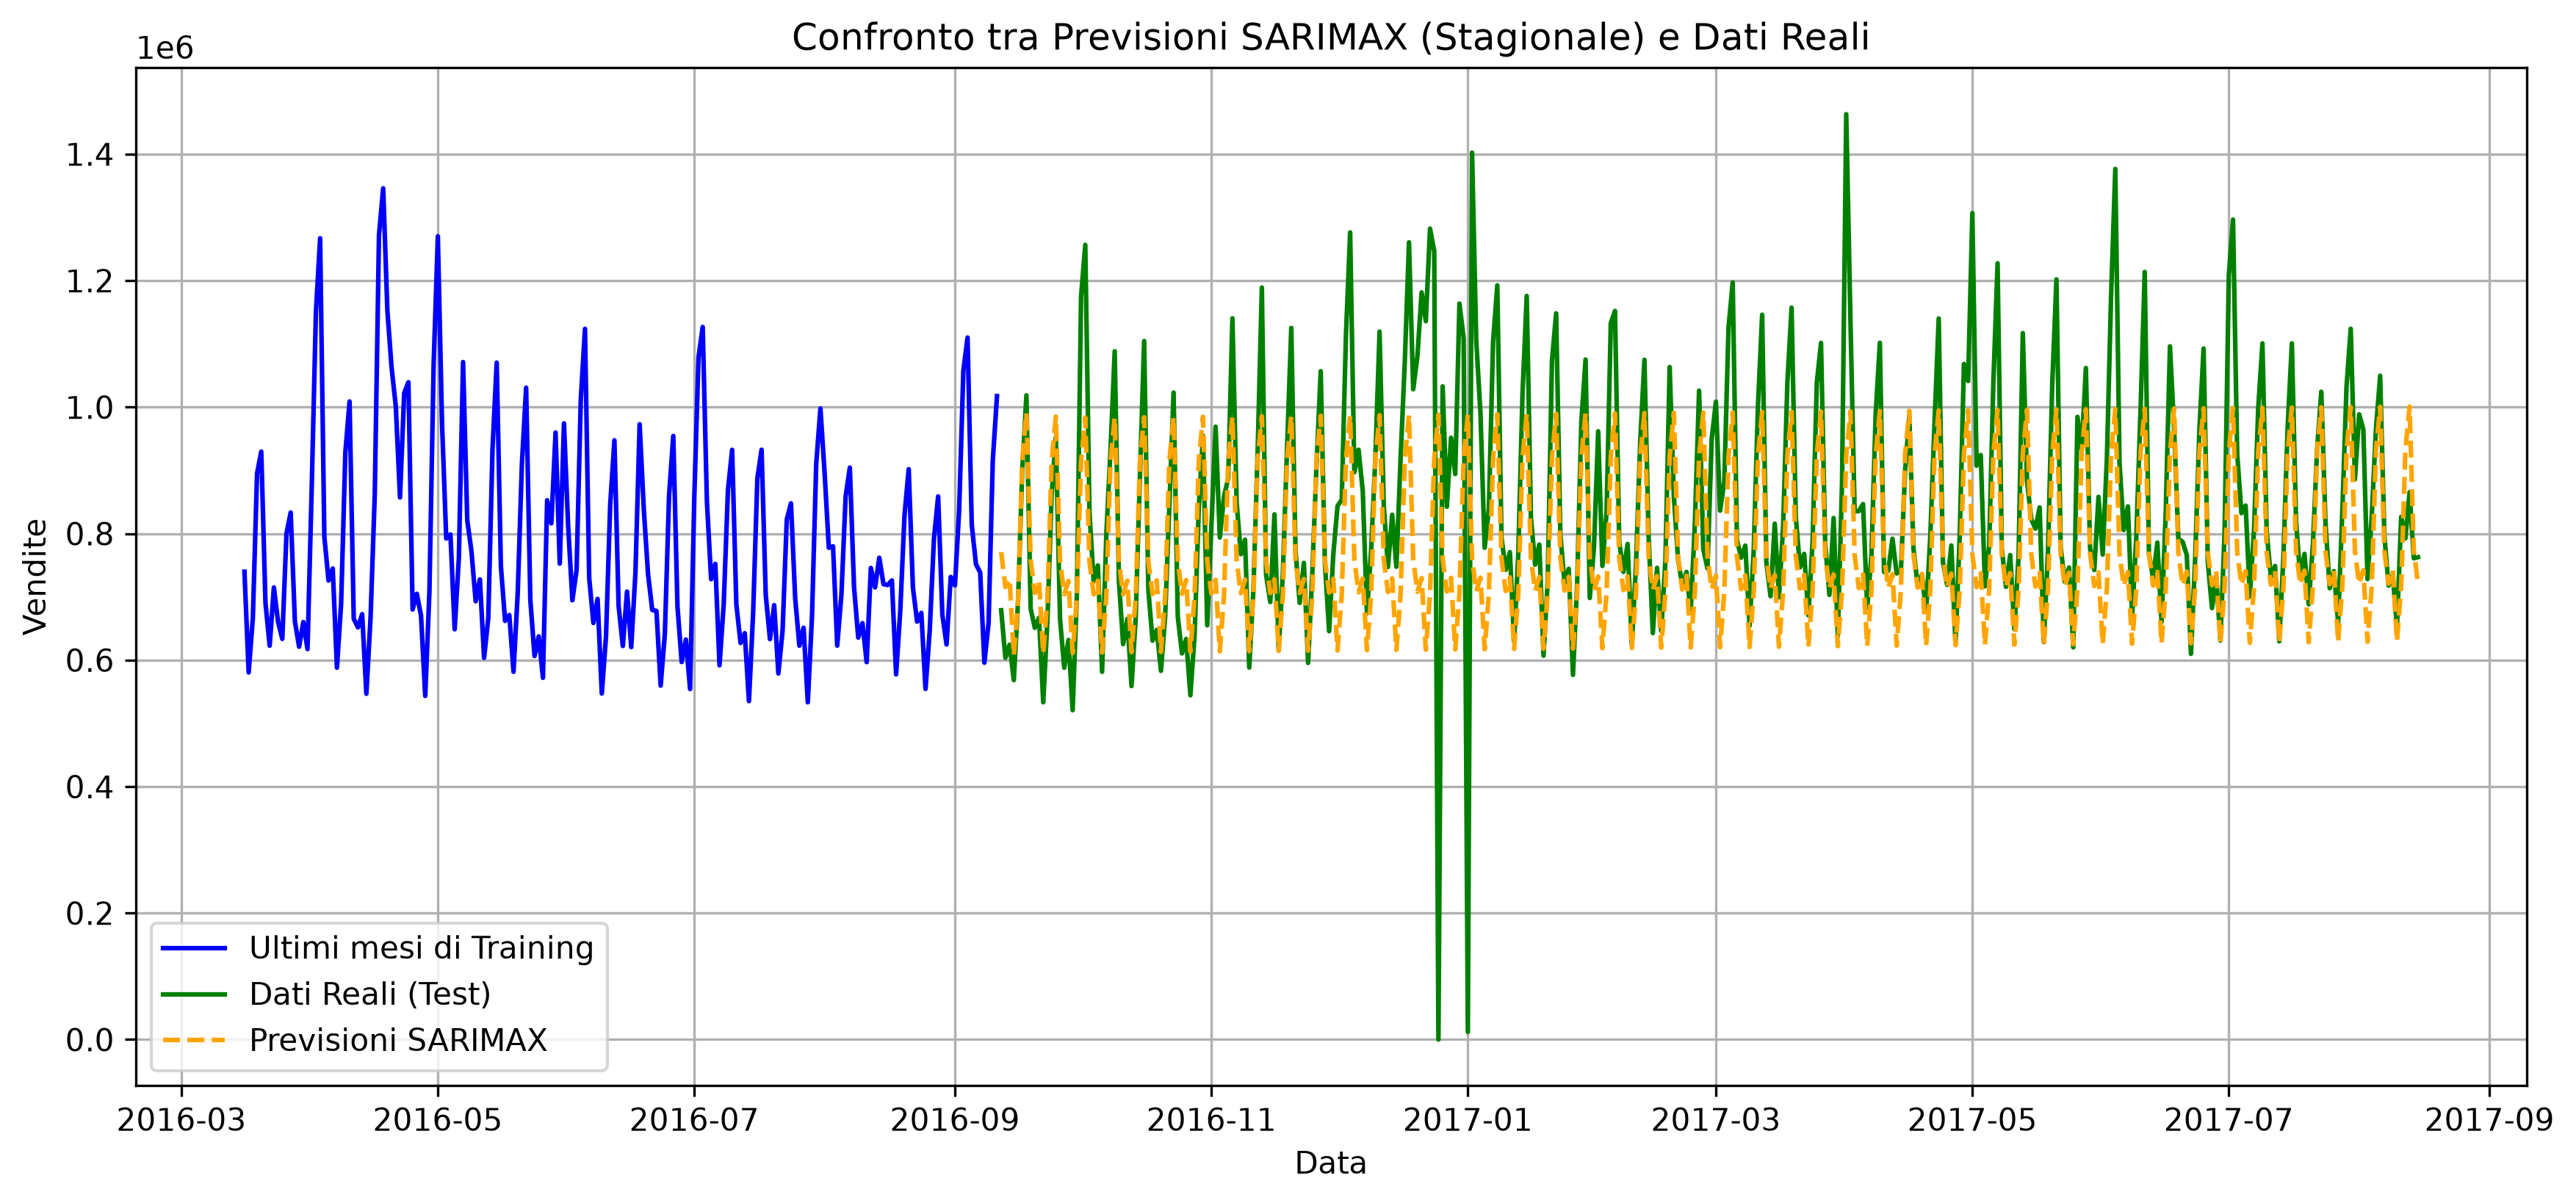
\includegraphics[width=\textwidth]{forecasting/images/fig03_previsioni_sarimax.png}
    \caption{Confronto grafico tra le previsioni generate dal modello SARIMAX stagionale (linea arancione tratteggiata) e i dati reali del set di test (linea verde).}
    \label{fig:previsioni_sarimax_tesina}
\end{figure}

Come si evince dall'analisi visiva del grafico di confronto (Figura~\ref{fig:previsioni_sarimax_tesina}), l'integrazione della componente stagionale settimanale ha consentito al SARIMAX di superare il limite strutturale dell'appiattimento tipico dei modelli ARIMA lineari puri, permettendo alla curva previsionale di seguire dinamicamente le oscillazioni cicliche della domanda commerciale.

% =============================================================================
\section{Analisi Diagnostica dei Residui e Conclusioni}
\label{sec:diagnostica_forecasting}
% =============================================================================

Al fine di validare rigorosamente la correttezza statistica e l'assenza di distorsioni sistematiche nel modello SARIMAX sviluppato, è stata condotta un'analisi approfondita sui residui di stima.

\begin{figure}[H]
    \centering
    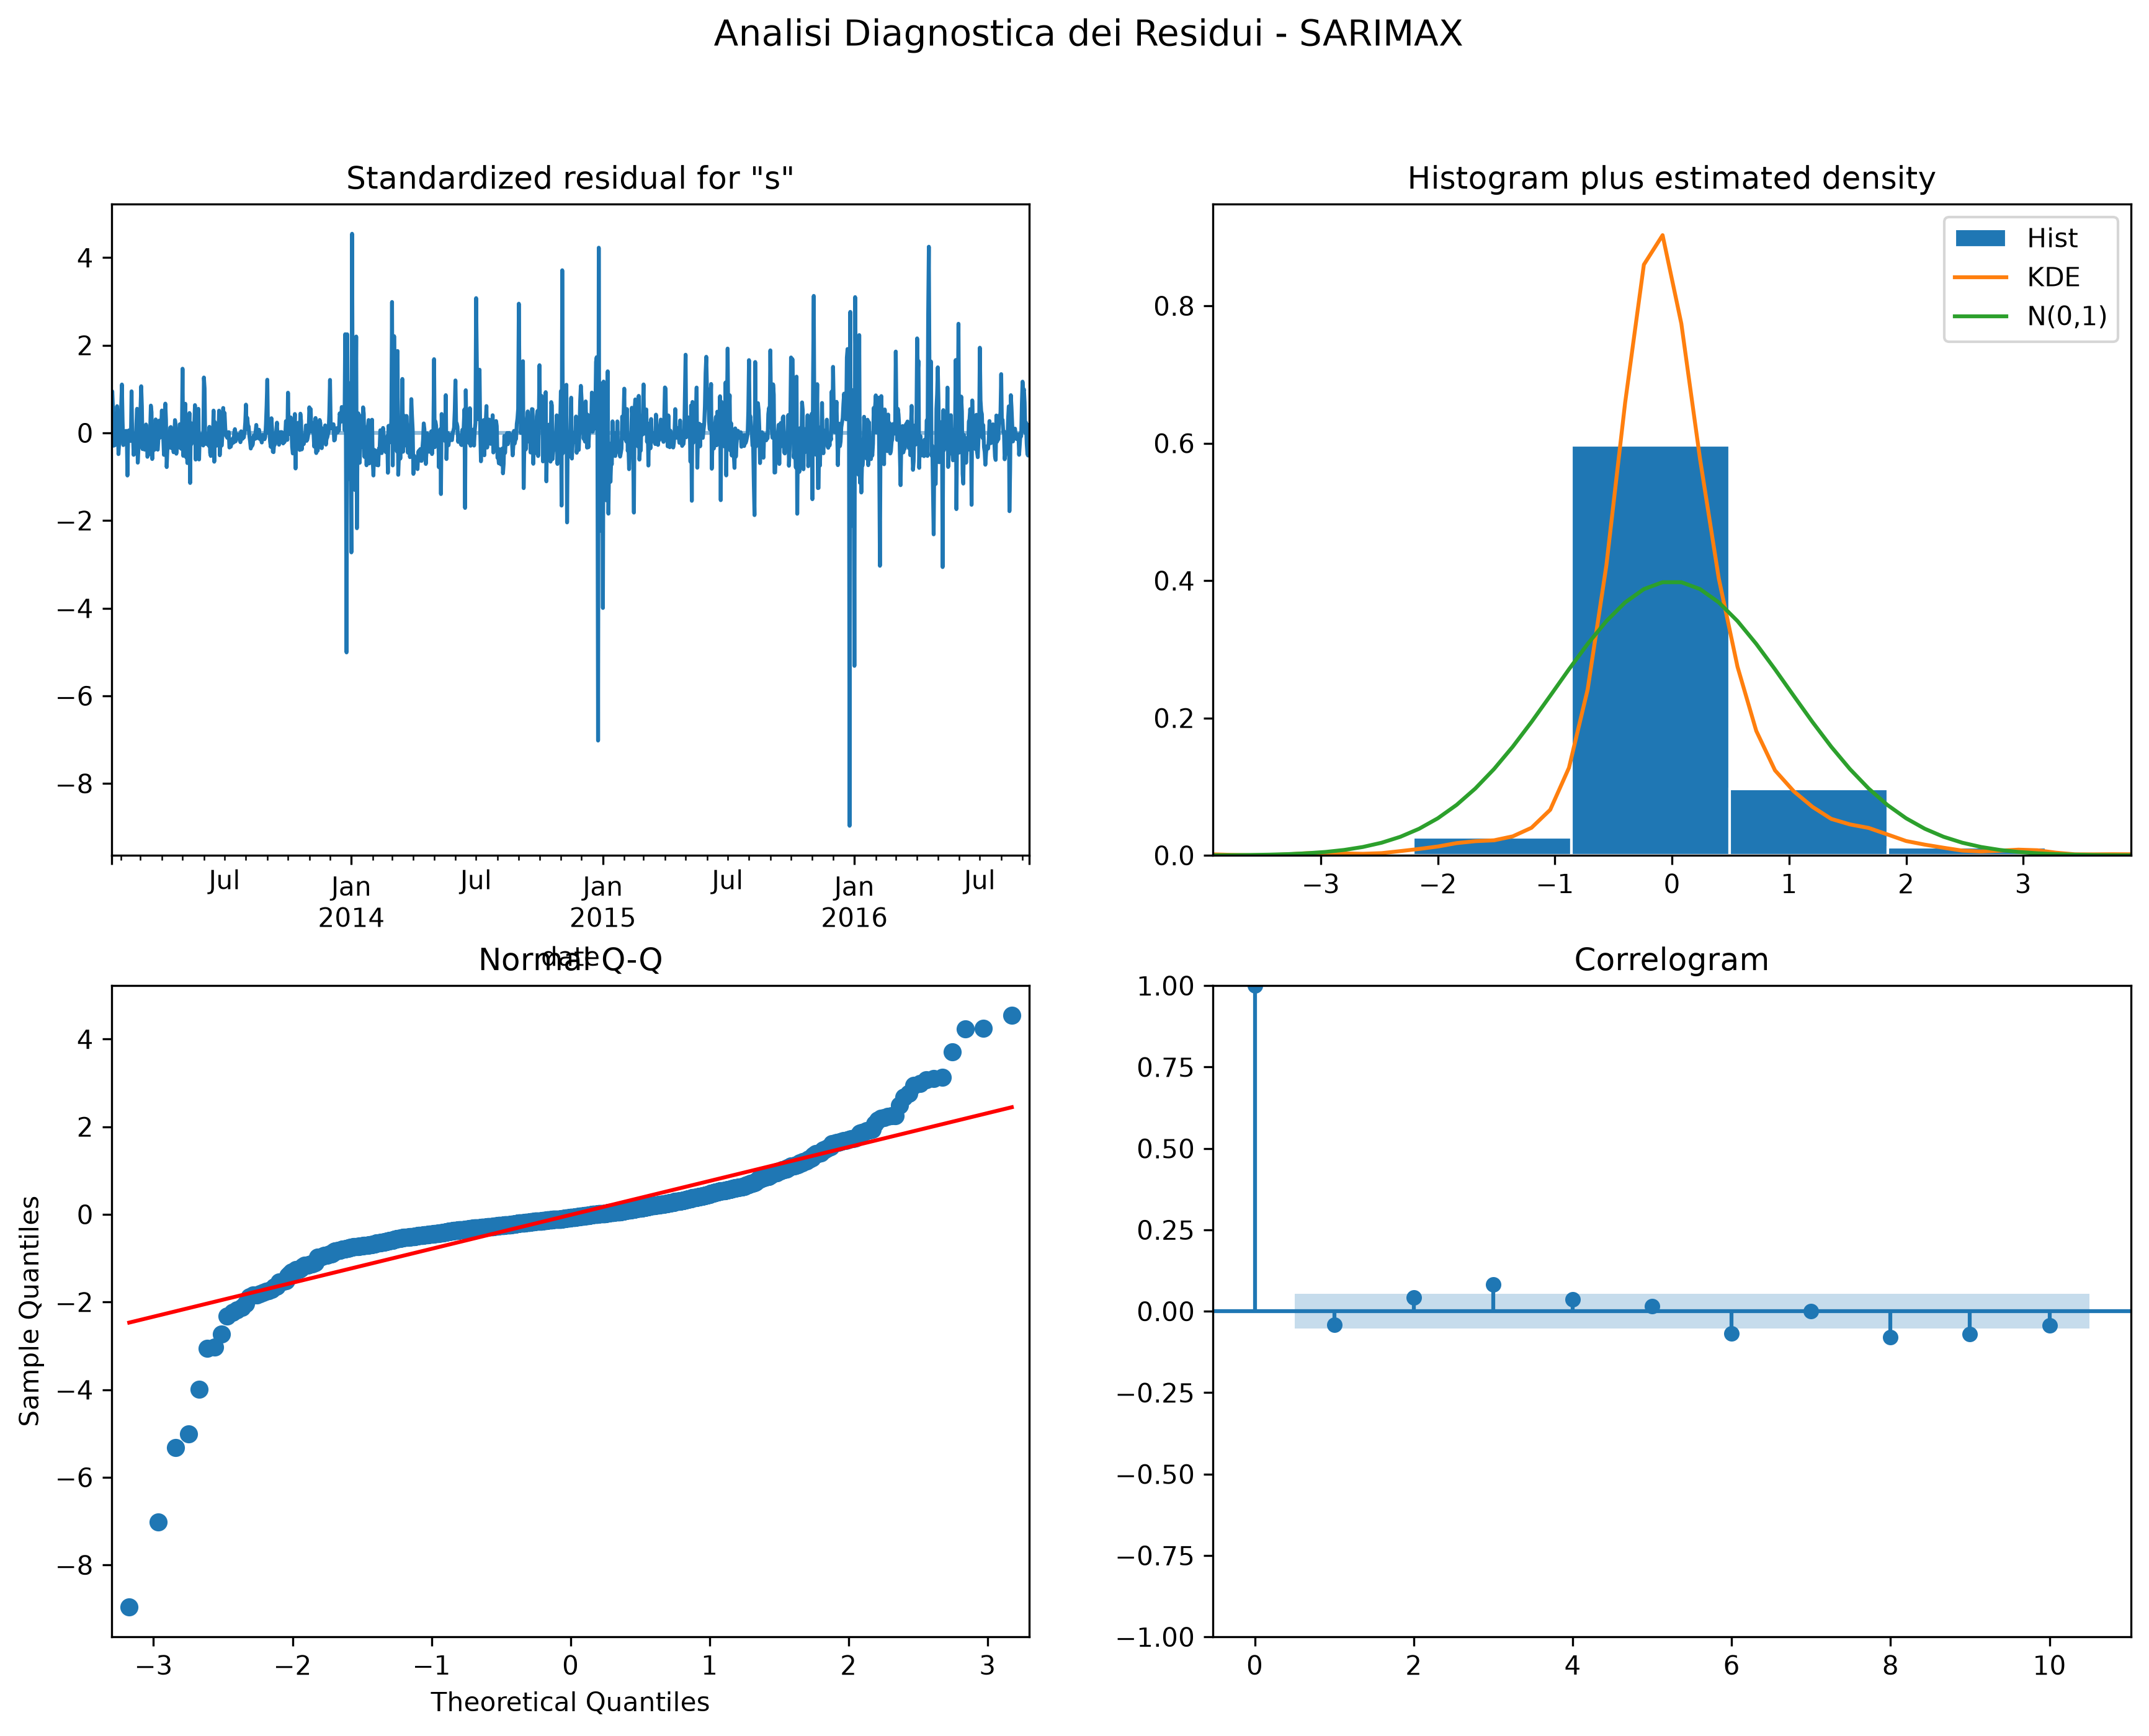
\includegraphics[width=\textwidth]{forecasting/images/fig04_diagnostica_residui.png}
    \caption{Analisi diagnostica completa dei residui del modello SARIMAX: andamento standardizzato nel tempo, istogramma con stima di densità KDE, grafico Q-Q Normale e correlogramma ACF.}
    \label{fig:diagnostica_residui_forecasting}
\end{figure}

L'esame dei quattro pannelli diagnostici (Figura~\ref{fig:diagnostica_residui_forecasting}) permette di trarre le seguenti conclusioni:
\begin{enumerate}
    \item \textbf{Residui Standardizzati nel Tempo:} Gli errori fluttuano attorno a una media costante pari a zero, con una varianza complessivamente omogenea, pur risentendo di lievi sussulti in corrispondenza di shock commerciali atipici.
    \item \textbf{Istogramma e Densità (KDE):} La distribuzione empirica dei residui si adatta in modo eccellente alla curva di densità normale teorica ($\mathcal{N}(0,1)$), confermando l'ipotesi di normalità degli errori.
    \item \textbf{Grafico Q-Q Normale (\emph{Quantile-Quantile}):} I quantili dei residui seguono in modo coerente la bisettrice teorica di riferimento, salvo lievi scostamenti sulle code esterne tipici dei dati commerciali reali ad alta intensità.
    \item \textbf{Correlogramma (ACF):} L'funzione di autocorrelazione dei residui mostra che tutti i coefficienti associati ai vari lag rientrano interamente all'interno della fascia di confidenza statistica (area azzurra), attestando l'assenza di autocorrelazione residua e confermando che il modello SARIMAX ha catturato in modo esaustivo la struttura dinamica della serie temporale.
\end{enumerate}

In sintesi, i risultati ottenuti confermano che l'approccio modellistico basato su SARIMAX rappresenta una soluzione robusta, interpretabile e altamente affidabile per il forecasting dei volumi di vendita nel settore retail.